\section{Libraries} \label{sec:libraries}
\noindent
KitFox provides a standardized method to integrate various implementations of physical modeling tools.
In KitFox, standard classes called \emph{libraries} are created, where each library hosts different type of model; \emph{energy}, \emph{thermal}, \emph{reliability libraries}:
\begin{itemize}
\item{\textbf{Energy Library}\\
- Estimating per-access energy of different access types (e.g., logical switching, read, write, etc.)\\
- Area calculation based on circuit-level models\\
- Runtime update of variables (e.g., voltage, clock frequency, etc.)} 
\item{\textbf{Thermal Library}\\
- Floor-planning and power-grid mapping\\
- Calculation of steady-state or transient temperatures\\
- Runtime update of variables (e.g., ambient temperature, coolant flow rate, etc.)} 
\item{\textbf{Reliability Library}\\
- Calculation of transient failure rates based on operating conditions\\
- Runtime update of variables (e.g., temperature, voltage, etc.)}
\end{itemize} 

\noindent
The following is the baseline model library class that derives different library classes:
{
\fontsize{10pt}{11pt}\selectfont
\begin{alltt}
/* Base Library Class defined in library.h */
class model_library_t \{
public:
    model_library_t(pseudo_component_t *PseudoComponent, int Type);
    virtual ~model_library_t();

    /* A model library must support runtime update of parameters.
       This function is also used as a callback function when new data are inserted
       into pseudo component queues. */
    virtual void update_library_variable(int type, void *Value, bool isLibraryVariable=false)=0;

    /* Initialize a subclass model. */
    virtual void initialize(void)=0;

    /* Type: energy, thermal, or reliability model */
    int type;

protected:
    /* The pseudo component that this model library is linked at. */
    pseudo_component_t *pseudo_component;
\};
\end{alltt}
}

\subsection{Energy Library} \label{subsec:energy_library}
\noindent
Power modeling tools are encapsulated as the subclass of the energy library. 
Power (or energy) is characterized at architecture-level components whose circuit-level behaviors are estimated from supported tools, based on technology parameters and architectural component configurations.
For each modeled component in the simulator, a model of the energy library estimates per-access dynamic energies of distinct access types (e.g., read/write, logical switching, etc) and leakage power.
Total dynamic energy is calculated by multiplying estimated per-access energies with corresponding types of access counters that can be collected from microarchitecture simulations.
Leakage power is exponentially dependent on temperature states, and it requires thermal analysis for accurate power modeling.
The following is the definition of the energy library class that hosts power modeling tools.

{
\fontsize{10pt}{11pt}\selectfont
\begin{alltt}
/* Energy Library defined in library.h */
class energy_library_t : public model_library_t \{
public:
    energy_library_t(pseudo_component_t *PseudoComponent, int Type);
    virtual ~energy_library_t();

    /* Calculate unit energy per access. */
    virtual unit_energy_t get_unit_energy(void)=0;

    /* Calculate TDP power. */
    virtual power_t get_tdp_power(Kelvin MaxTemperature=373.0)=0;

    /* Calculate runtime power. */
    virtual power_t get_runtime_power(Second Time, Second Period, counter_t Counter)=0;

    /* Calculate area (if available). */
    virtual MeterSquare get_area(void)=0;

    /* Type: specific energy library model (e.g., McPAT) */
    int type;
\};
\end{alltt}
}

\noindent
For each model being integrated into KitFox, a \emph{wrapper} class is created. 
The wrapper class is defined as the subclass of one of the library classes.
It includes header/source files of the tool to be integrated and re-defines the usage of the model according to the virtual functions of the corresponding library class.
Thus, the models of the same library type can be used in the identical way.
The following is the example of McPAT wrapper class being defined as the subclass of the energy library.

{
\fontsize{10pt}{11pt}\selectfont
\begin{alltt}
/* McPAT Wrapper Class */
class energylib_mcpat : public energy_library_t \{
public:
    energylib_mcpat(pseudo_component_t *PseudoComponent);
    ~energylib_mcpat();

    /* Virtual functions of base classes */
    virtual void initialize();
    virtual unit_energy_t get_unit_energy();
    virtual power_t get_tdp_power(Kelvin MaxTemperature=373.0);
    virtual power_t get_runtime_power(Second Time, Second Period, counter_t Counter);
    virtual MeterSquare get_area();
    virtual bool update_library_variable(int Type, void *Value, bool IsLibraryVariable=false);

private:
    /* McPAT input classes */
    ParseXML XML_interface;
    InputParameter input_p;
    ...

    /* McPAT library models */
    ArrayST *McPAT_ArrayST;
    dep_resource_conflict_check *McPAT_dep_resource_conflict_check;
    ...

    /* Tuning parameters used in the wrapper class */
    int energy_model, energy_submodel;
    double clock_frequency;
    double energy_scaling, area_scaling, scaling;
    ...
\};
\end{alltt}
}

\subsection{Thermal Library} \label{subsec:thermal_library}
\noindent
Temperature modeling tools are encapsulated as the subclasses of the thermal library.
Temperature is characterized at the package level.
A processor package is represented as the stack of layers with thermal grids.
Each thermal grid cell is expressed as a thermal RC connection.
Calculating thermal field over a processor package is equivalent to solving the differential equations of this thermal RC network.
Components representing a processor on the die are organized and represented by \emph{floorplans}.
Each floorplan component represents a set of microarchitectural units, where the power dissipation of each unit is estimated from the linked energy library model and microarchitectural timing simulation.
The power estimates of floorplans are supplied to a gridding process that calculates the power at each cell in a finer resolution (configurable).
This fine-grained power grid is the input to the thermal model that computes the temperature field over this grid.
Changes in temperature are coupled to leakage power creating a feedback loop between the energy and thermal libraries.

{
\fontsize{10pt}{11pt}\selectfont
\begin{alltt}
/* Thermal Library defined in library.h */
class thermal_library_t : public model_library_t \{
public:
    thermal_library_t(pseudo_component_t *PseudoComponent, int Type);
    virtual ~thermal_library_t();

    /* Calculate transient or steady-state temperature. */
    virtual void calculate_temperature(Second Time, Second Period)=0;

    /* Returns 3D temperature grid stack of power source layers. */
    virtual grid_t<Kelvin> get_thermal_grid(void)=0;

    /* Returns representative floorplan temperature.
    virtual Kelvin get_floorplan_temperature(Comp_ID ComponentID, 
                                             int Type=KITFOX_TEMPERATURE_MAPPING_UNKNOWN)=0;

    /* Returns point temperature. */
    virtual Kelvin get_point_temperature(Meter X, Meter Y, Index Layer)=0;

    /* Map floorplan power. */
    virtual void map_floorplan_power(Comp_ID ComponentID, power_t FloorplanPower)=0;

    /* Add floorplan. */
    void add_floorplan(std::string ComponentName, Comp_ID CompnentID);

    /* Returns total number of floorplans. */
    const Index get_floorplan_counts(void);

    /* Returns a pseudo component ID of ComponentName. */
    const CompID get_floorplan_id(std::string ComponentName);
    const char* get_floorplan_name(Comp_ID ComponentID);

    /* Returns ith pseudo component in the map. */
    const Comp_ID get_floorplan_id(unsigned i);

    /* Type: specific thermal library model (e.g., HotSpot) */
    int type;

private:
    std::map<std::string, Comp_ID> floorplan_name_map;
    std::map<Comp_ID, std::string> floorplan_id_map;
\};
\end{alltt}
}

\subsection{Reliability Library} \label{subsec:reliability_library}
\noindent
Gradual device wear leads to permanent failures.
Phenomena that lead to device wear include negative bias temperature instability (NBTI), hot carrier injection (HCI), time-dependent dielectric breakdown (TDDB), etc.
KitFox utilizes detailed interactive physics behaviors to calculate failure rates and predict lifetime reliability.
Transient failure rates are calculated with respect to time-varying stress conditions including voltage and thermal stresses.

{
\fontsize{10pt}{11pt}\selectfont
\begin{alltt}
/* Reliability Library defined in library.h */
class reliability_library_t : public model_library_t \{
public:
    reliability_library_t(pseudo_component_t *PseudoComponent, int Type);
    virtual ~reliability_library_t();

    /* Calculate failure rate. */
    virtual Unitless get_failure_rate(Second Time, Second Period, Kelvin Temperature, 
                                      Volt Vdd, Hertz ClockFrequency)=0;

    /* Type: specific thermal library model */
    int type;
\};
\end{alltt}
}

\subsection{Physical Interactions} \label{subsec:physical_interactions}
\noindent
In KitFox framework, multiple physical models are concurrently simulated, and their interactions are captured at user-defined sampling rate, typically invoked by cycle-level microarchitecture simulation models.
Figure \ref{fig:interactive_simulation} depicts an architecture-level abstraction of interactions between multiple physical properties and associated models.
Execution of workloads through microarchitecture simulation generates switching activities of functional components. 
Architectural activities are represented with access counters and used to calculate dynamic power dissipation of modeled components.
Leakage power is estimated by assuming a constant temperature during the sampling interval.
Power results are mapped onto user-created thermal floorplans, and temperature is calculated based on the spatial distribution of input power and thermal grid states.
Changes in temperature incur thermal-leakage power feedback, and recalculated leakage power is used for temperature calculation in the next sampling period. 
Reliability characteristics (i.e., failure rates) of modeled components are calculated with respect to time-varying operating conditions (i.e., voltage and thermal stresses).
The chain of interactions create a loop and is repeated at every sampling interval.
Execution controls such as voltage and frequency scaling may intervene in this chain of events and dynamically change operating conditions and resulting behaviors of physical phenomena.

\begin{figure}[h]
\centering
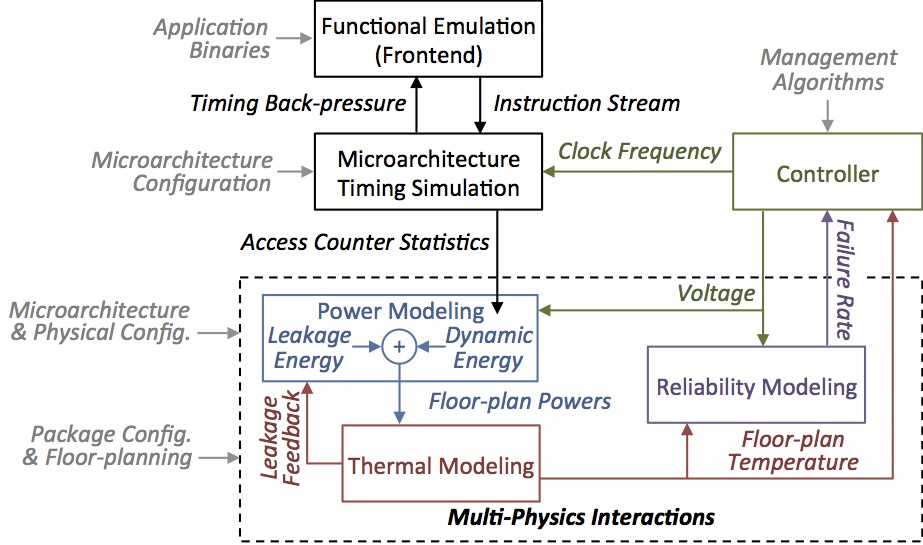
\includegraphics[width=0.6 \textwidth]{figures/interactive_simulation.jpg}
\caption{Architecture-level abstraction of interactions between multiple physical properties and microarchitecture. These interactions are captured concurrently during runtime simulation.}
\label{fig:interactive_simulation}
\end{figure}

\pagebreak
